\documentclass[a4paper,10pt]{article}
\usepackage[margin=1in]{geometry}
\usepackage{enumitem}
\usepackage[pdftex]{graphicx}
\usepackage{bbm}
\usepackage{amsfonts}
\usepackage{amsthm}
\usepackage{subfigure}

\theoremstyle{definition}
\newtheorem{defn}{Definition}
\newtheorem{obs}{Observation}
\begin{document}
\subsection*{5-9-notes}
\begin{enumerate}
\item \emph{Simulating data:}  With the coefficients of the generalized linear model set to 1, for each of the 3 linear models ($B_a=B_b=B_c=1$), created a set of 50 patients, chose covariate values for the 50 patients, and for each patient, obtained a sample of $a, b, c$.  (actually, so that there was no noise when simulating data, deterministically calculated for each patient $\tilde{\mu_a}|\tilde{x}, \tilde{\mu_b}|\tilde{x}, \tilde{mu_c}|\tilde{x}$, which is the conditional expectation of $a, b, c$ given a $\tilde{x}$, respectively, and used that.  For now, only using 1 covariate.  Plotted a scatterplot of the single covariate value $\tilde{x}$ of each patient vs their value of $a, b, c$.  See Figure 1.  There should be a (general) linear relationship between the covariate value and $a, b, c$.

\item \emph{Recovering parameters used to simulate data: }  Took those samples, used them as observed data, and plotted distributions of $B_a, B_b, B_c$.  Since those samples were generated from a model where  $B_a=B_b=B_c=1$, the posterior of  $B_a, B_b, B_c$ should be centered around 1.  See Figure 2.

\item Beta distributions for each data point should probably have the same dispersion parameter(shared)

\item We decided it's okay to have independent models for each treatment.

\end{enumerate}

\begin{figure}
\begin{center}
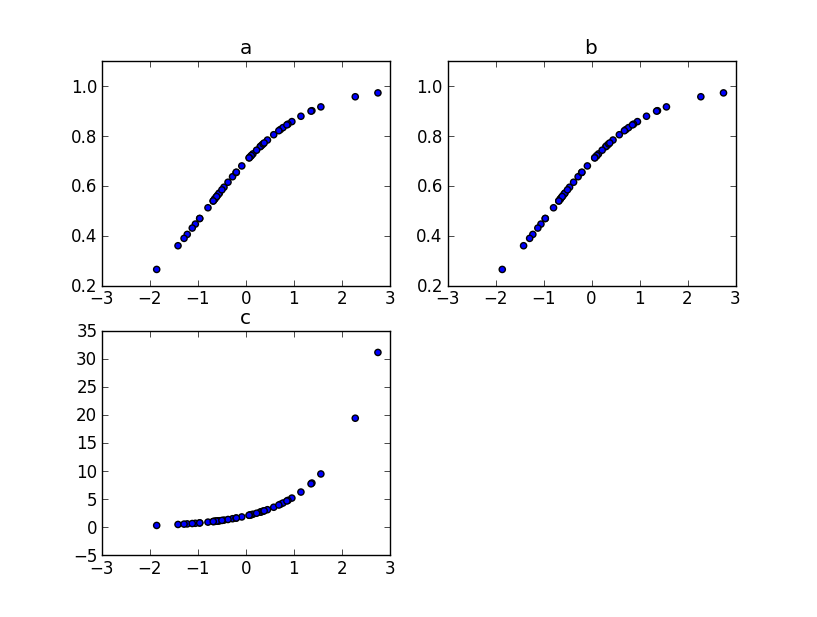
\includegraphics[width=5in, height=4in]{/Users/glareprotector/prostate_git/glare/bin/abc_vs_covariates.png}
\caption{plots of a,b,c vs covariate value with $B_a=B_b=B_c=1$}
\end{center}
\end{figure}

\begin{figure}
\begin{center}
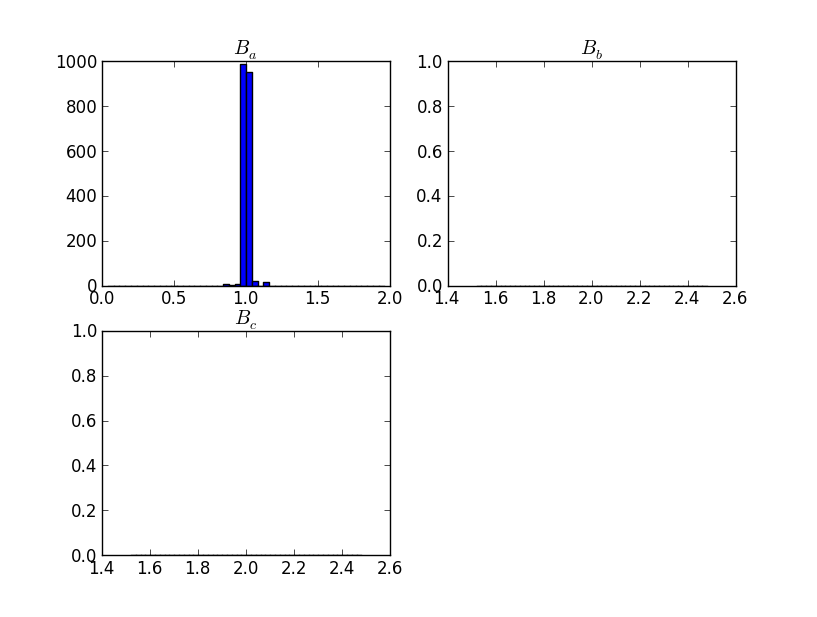
\includegraphics[width=5in, height=4in]{/Users/glareprotector/prostate_git/glare/bin/Bs.png}
\caption{Distribution of $B_a, B_b, B_c$ using the simulated data}
\end{center}
\end{figure}



\end{document}